Libraries, structured and curated collections of informational resources, play a key role in preserving the collective memory of the human civilisation and its heritage. The resources they store take various structural (manuscripts, media, articles) and semantic (historic records, research, literature) forms and are made available to either the general public or more finer-grained user groups.

With the advent of the \gls{www} in the late 20th century, libraries were among the first applications of the new online technologies, giving rise to \emph{digital} libraries. It can be argued that the \gls{www} as a whole represents in itself a library; still, discrete instances can maintain the structural and semantic differentiation mentioned previously and can better target various user groups, catering to their specific needs.

As the \gls{www} was the driving factor behind the digitisation of libraries, the progress of scholarship and scientific research played an important role in the evolution of digital libraries, a number of aspects being factored into this. First, research funding has greatly increased, as presented in Fig. \ref{fig:fundig} and, as a direct result, the number of outputs, such as monographs, journal articles or theses, has increased (see Fig. \ref{fig:nopublications}). This impacted digital libraries which now need to be able to manage a larger influx of new content while ensuring its proper dissemination across stakeholders. 
\begin{figure}[ht!]
\centering
\begin{subfigure}{0.9\textwidth}
  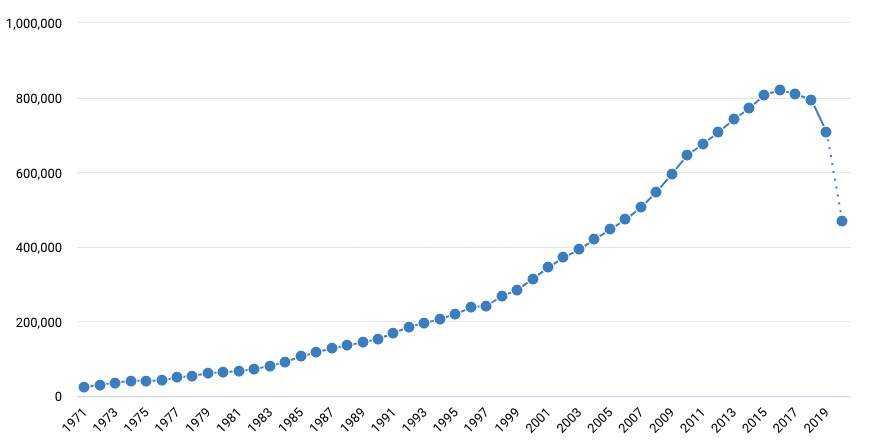
\includegraphics[width=1\linewidth]{figures/no_grants.png}  
  \caption{Evolution of number of research grants since 1971. Data since 2018 is incomplete.}
  \label{subfig:grants}
\end{subfigure}
\begin{subfigure}{0.9\textwidth}
  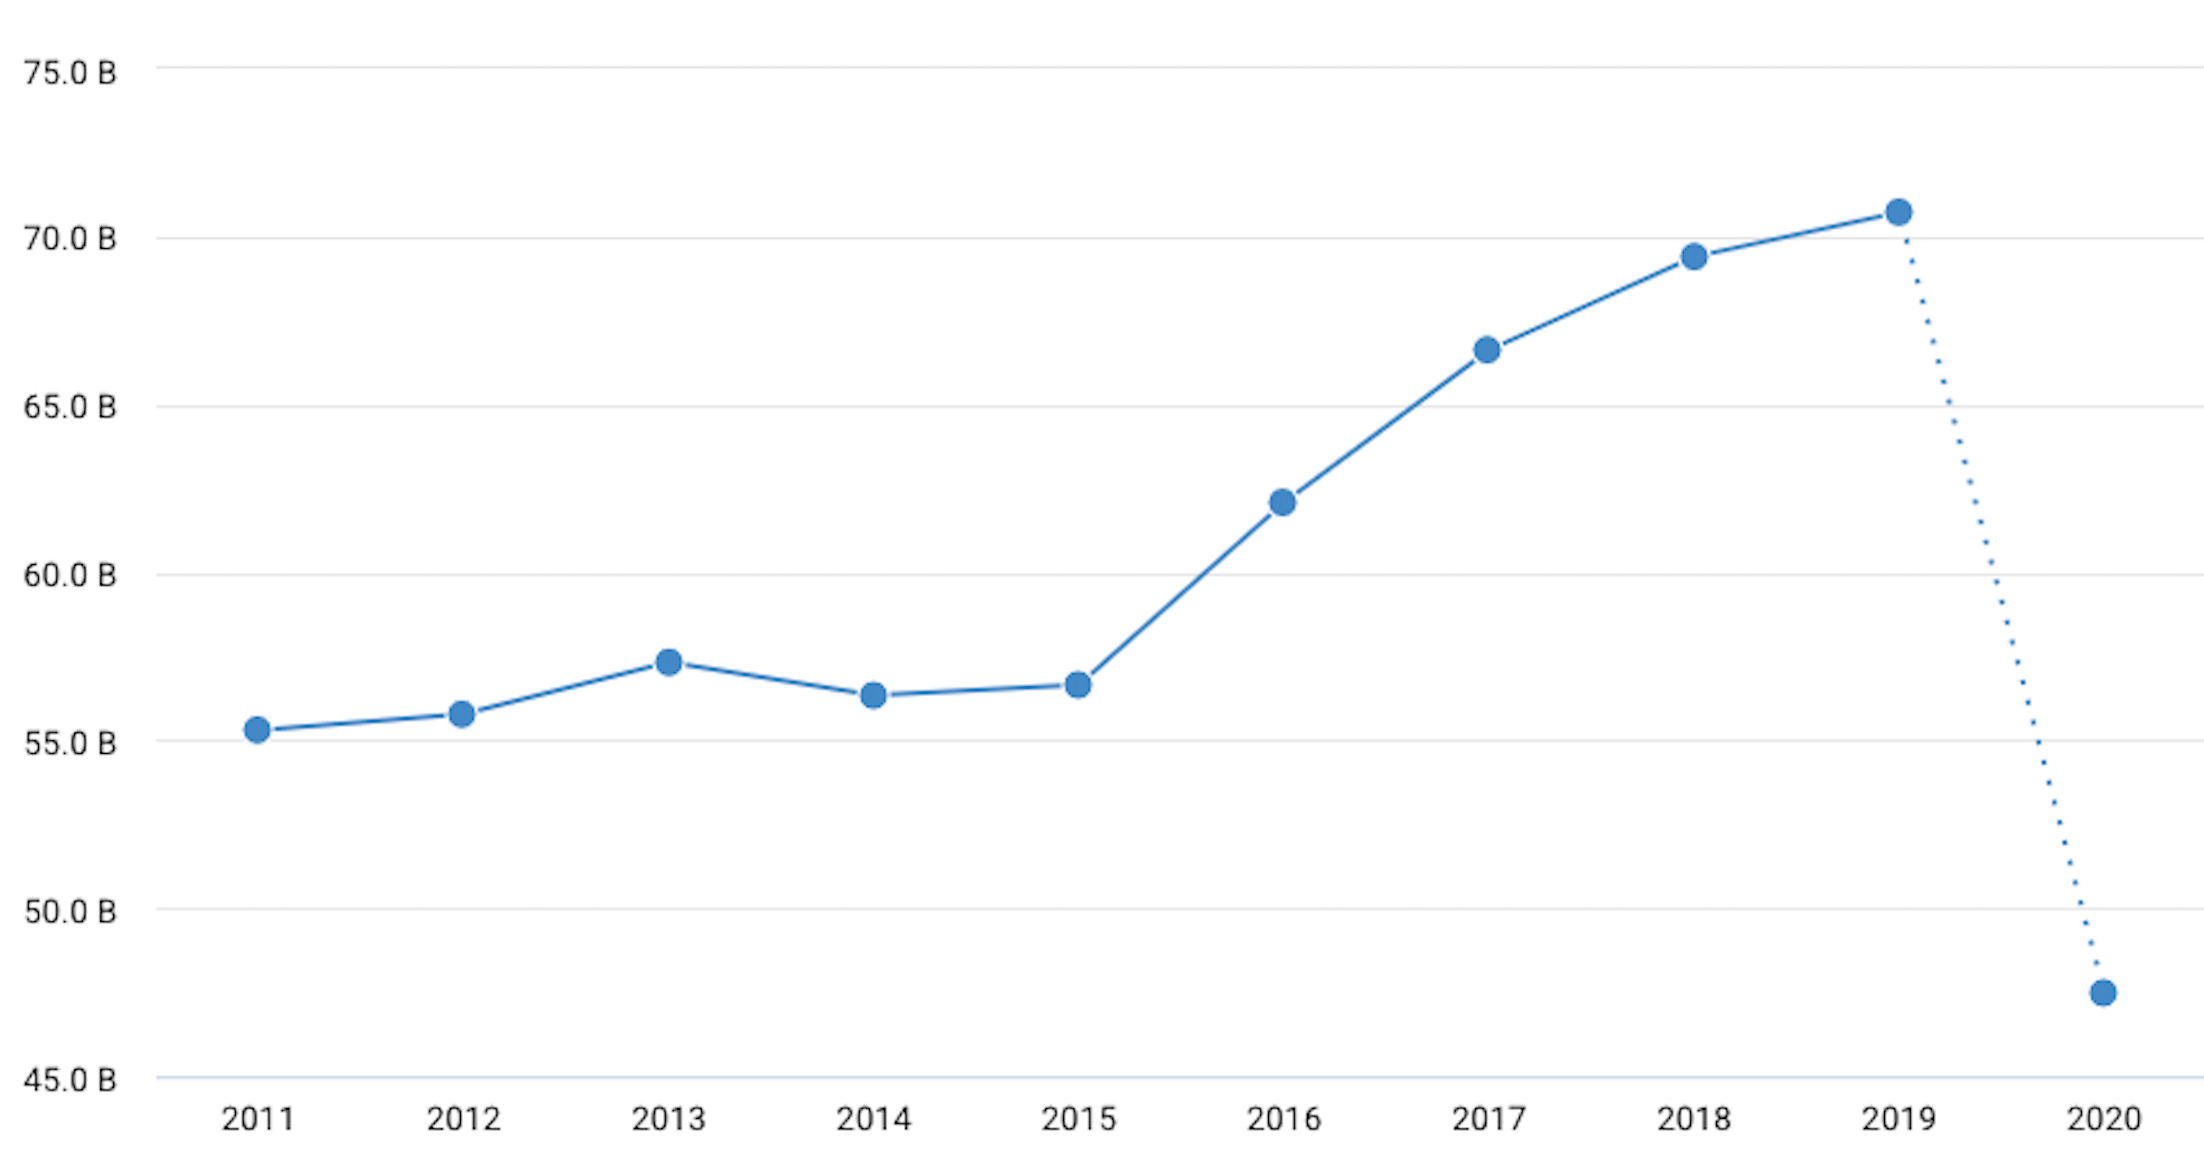
\includegraphics[width=1\linewidth]{figures/funding.png}  
  \caption{Evolution of total amount of research grants since 2011, in pounds sterling. Data for 2020 is incomplete.}
  \label{subfig:grantstotal}
\end{subfigure}
\caption{Evolution of research funding; source \url{https://app.dimensions.ai}.}
\label{fig:fundig}
\end{figure}

\begin{figure}[ht!]
\centering
  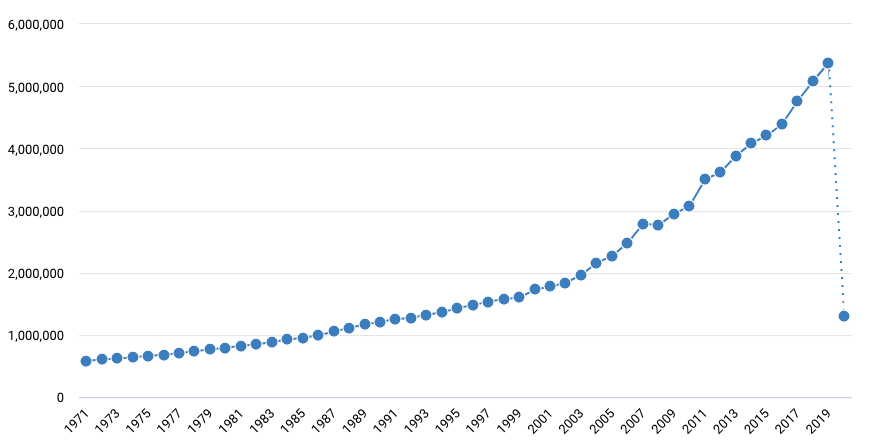
\includegraphics[width=1\linewidth]{figures/publications.png}  
  \caption{Evolution of number of research publications, data since 2019 is incomplete; source \url{https://app.dimensions.ai}.}
  \label{fig:nopublications}
\end{figure}

Second, a number of significant events in the area of research and scholarly communications have taken place; two of these are of interest.

The \emph{\gls{oa}} reforms came to prominence along with digital libraries; as the medium for disseminating research switched from physical (paper journals or monographs) to digital, researchers questioned the suitability of the traditional business plans of publishers (e.g., Springer Nature or Elsevier), which could no longer fully justify the costs inquired for typesetting and printing, among others. \gls{oa} is one proposed way of resolving this, its aim being to shift the costs of publishing from being supported by consumers to being supported by producers (i.e., researchers wishing to disseminate their work, or, most often, their funders). \gls{oa} can be practically implemented in a number of ways, but of interest here are the following:
\begin{itemize}
    \item Gold: the article is published as \gls{oa} in a journal pending the publication of a fee by the authors and using a licencing model that places no barriers towards sharing and reuse.
    \item Green: while the reviewed, typeset and copy-edited article is published by the journal under its own terms, the authors are allowed to freely share their own versions using other means.
\end{itemize}
An obvious platform for depositing both these types of \gls{oa} manuscripts is the digital library managed by the authors' affiliated institutions. In \cite{oa} the authors measured that between 2000 and 2016 over 4 million gold \gls{oa} have been published and over 2 million green \gls{oa} versions have been deposited in repositories.

\gls{oa} is a subset of a much complex movement, \emph{open science}, which aims at making all research outputs and workflows publicly available; this includes, but is not limited to, tools and applications used in research, methods for measuring the impact of published results, or policies allowing a wider audience to consume and produce research\footnote{An example here is the concept of \emph{citizen science}, which aims at involving amateurs in research by allowing them, among others, to perform repetitive task which do not require in-depth domain knowledge.}.

The \emph{reproducibility crisis} is a phenomenon generated by a number of research studies that failed to \emph{replicate}, other researchers not being able to verify the claims of the original authors by repeating similar experiments. An infamous such example is a paper\footnote{Wakefield et. al. (1998) \emph{RETRACTED: Ileal-lymphoid-nodular hyperplasia, non-specific colitis, and pervasive developmental disorder in children}} published in 1998 in The Lancet, which linked the measles, mumps and rubella vaccine to colitis and autism spectrum disorders in children. The paper was lately retracted, due to evidence of fraud, conflicts of interest and manipulation of data. The literature currently documents multiple instances of studies that exhibit reproducibility or replication\footnote{It is widely accepted that \emph{reproducibility} is the act of reaching original research result by using the same research materials (data, software, instruments), while \emph{replicability} uses different inputs (e.g., a new set of patients for a clinical study) in order to reach similar results\cite{patil}.} issues, due to, among others, technical, methodology or workflow faults (see, for example \cite{eklund,seekblastn}).

As a result of this crisis, the world of research focused in latest years on ensuring that published scientific result are accompanied by all the required artefacts (e.g., data, software, protocols) necessary to allow other researchers to fully verify the claims of the original authors. This move was also formalised by both research funding bodies\cite{h2020,nih} and publishers\cite{scidat,elsdat}, such that good practices are enforced across the whole scientific community. This type of policies are part of the \emph{open data} movement, which along with \gls{oa} form the so-called \emph{democratic} school of thought in open science, which concerns itself with removing any barriers to accessing and reusing research.

For digital research libraries this meant, above everything, adapting to the new types of outputs; data sets or scientific software present new challenges, due to their structural and semantic particularities. Moreover, libraries need to ensure that all outputs generated by a scientific study are presented in a coherent and consolidated manner, in order to facilitate reproducibility. Assisting with reproducibility is a crucial dimension that needs to be considered by \emph{all} tools in the research ecosystem, as \emph{``expecting a researcher to reproduce either entirely or in part the outcomes of a large or costly study or data collection exercise is not reasonable''}\cite{oa} and thus, all possible forms of assistance, including those at the technological level, need to made available.

In \cite{oa} the authors note that \emph{``the reproducibility crisis is just one manifestation of a broken credit system where researchers are incentivised to publish positive results and suppress or disregard negative results''}; this comes to strengthen the motivations behind open science, and at the same time, suggests that the role of repositories is continuously expanding to include, for example, support for new types of outputs or novel methods of quantifying and qualifying the impact of research.

This thesis documents the evolution of digital libraries in light of the two challenges mentioned above and by describing how this suite of applications has overcome them by developing new features and workflows. It approaches this by considering the development of \emph{data repositories}, digital libraries aimed of hosting the new types of outputs mentioned above in general and research data in particular. For a considerable span of time, data repositories evolved in parallel with their more traditional counterparts, \glspl{ir}, archives of intellectual outputs of a research institution, most often a university. \glspl{ir} are a subset of digital libraries, as the latter could also hold content which is not scientific in nature, and, as opposed to data repositories, are more focused on scientific \emph{literature}, such as journal articles, monographs or theses. It is worth noting that across the thesis the term \emph{repository} is employed, due to its wide use in the field as a direct result of the spread of \gls{ir} solutions.

Nevertheless, in the last years, institutional, data, software and other scientific outputs repositories started to converge into unified solutions which can accommodate the disparate needs of researchers on one hand, and minimise the administrative work of librarians and technology teams on the other\footnote{The distinction between this two types of staff is beginning to fade, as librarians need to adapt to the new realities of the research ecosystem by including software-assisted workflows and tools in their craft; an example of this is the the Software Carpentry project at \url{https://software-carpentry.org/blog/2015/05/coding-for-librarians.html}.}. Thus, it can be argued that a new type of platform, the \emph{research}, or, as \cite{cmu} designates it, \emph{comprehensive} repository is beginning to take shape, by taking advantage of both the strong points of each type of existing platform, and also of the opportunities offered by the new research ecosystem and evolution of technology in general.

Thus, Chapter \ref{ch:evolution} begins with a detailed description of data repositories and follows with a description of the reasons and means for merging all types of repository applications into generic research repositories. The next three chapters focus on the practical implementation of features and workflows which could benefit this type of software infrastructure, namely licencing solutions using blockchains and smart contracts (Chapter \ref{ch:blockchain}), data modelling using \gls{rdf} (Chapter \ref{ch:rdf}), and record migration and management solutions employing \gls{etl} pipelines. This is an attempt of employing tools and processes specific to software engineering, which are wide spread in other types of applications, to digital libraries, with the aim of presenting a possible blueprint for the next generation research repository.